\begin{frame}
	\frametitle{Neal's Algorithm 8}
	\begin{itemize}
	    %\item Markov chain with permanent state $\mathbf c$ and $\boldsymbol\phi$ %(?)
		\item \textbf{Gibbs sampling} on the state, which is extended by the addition of $m$ \textbf{auxiliary parameters} \\
		    % No integration with respect $G_{0}$ is required
        \begin{center}
        	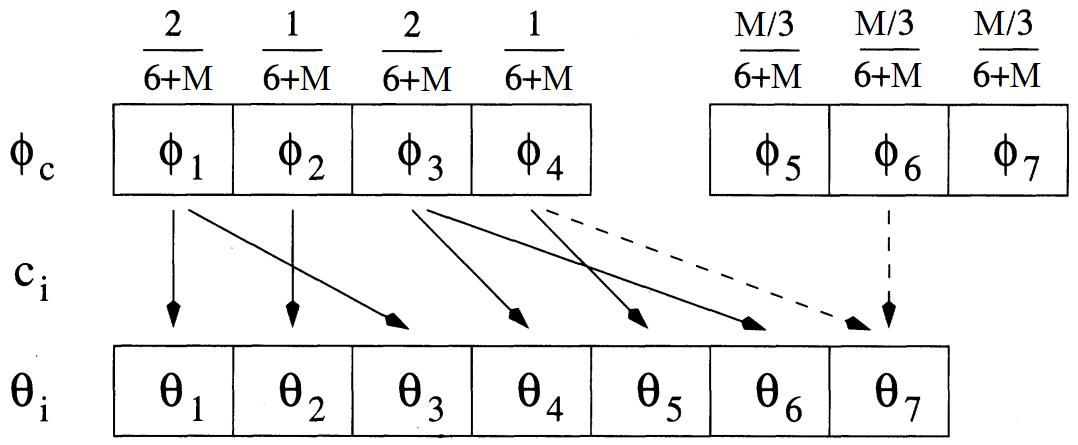
\includegraphics[scale=0.35]{etc/neal8.png}
        \end{center}
		
        \item Prior for $c_{i}$:
            \begin{align*}
            \hspace{-25pt}
            \vspace{-12pt}
                \text{If $c=c_j$ for some $j$: } \PP(c_i=c | \mathbf c_{-i}) &= \frac{n_{-i,c}}{n-1-M}  \\
                \PP(c_{i}\neq c_{j} \text{ for all } j) &=\frac{M }{n-1-M}  \Rightarrow 
                \begin{tabular}{c}
                \textbf{split} among the $m$ \\
                auxiliary parameters 
                \end{tabular}
            \end{align*}	
	\end{itemize}
\end{frame}


\begin{frame}
	\frametitle{Neal's Algorithm 8}
	Algorithm:
		\begin{itemize}
		    \item For $i= 1,\dots,n$: update $c_{i}$
		        \begin{itemize}
		            \item Sample auxiliary parameters: \begin{list}{$\circ$}{} 
		                \item $c_{i}=c_{j}$ for some $j\ \Rightarrow$ no connection \\
		                \item $c_{i}\neq c_{j} \ \Rightarrow$ association to one of $m$
		            \end{list}

		            The other $\phi$ values drawn from $G_{0}$
		            \item Draw $c_{i}$ as follows: %(by evaluating relative prob of these possibilities)
		            	\begin{displaymath}
		            	\hspace{-20pt}
		            	P(c_{i}=c | \mathbf c_{-i}, y_{i}, \phi_{1},...,\phi_{h}) \propto \begin{cases}  \frac{n_{-i,c}}{n-1-M}F(y_{i},\phi_{c}), & \mbox{for } 1 \leq c \leq k^{-} \\ \frac{M/m}{n-1-M}F(y_{i},\phi_{c}), & \mbox{for } k^{-}+1 < c \leq h
		            	\end{cases}
		            	\end{displaymath}
                    \item Discard values in $\boldsymbol\phi$ not associated to any $\theta_j$
                    
                \end{itemize}
        
            \item For $c \in \{c_{1},..,c_{n}\}$: update $\phi_{c}$ given $y_{i}$ such that $c_{i}=c$
		\end{itemize}
\end{frame}


\begin{frame}
	\frametitle{Advantages}
	\begin{itemize}
	    \item  Models with non-conjugate priors
	    \item As $m \rightarrow +\infty$ it approaches Algorithm 2 but equilibrium distribution is exact 
	    \item More efficient than similar algorithms (e.g. no-gaps) %not reduced prob to create new cluster
	    \item Hierarchical extensions
	\end{itemize}

		
\end{frame}

	

\begin{frame}
	\frametitle{Stick-Breaking Priors}
	$$\mathscr{P}(\cdot)= \sum\limits_{k=1}^N
	\mathit{p_{k}}\delta_{Z_{k}}(\cdot)$$
	with:
	\begin{itemize}
		\item $Z_k \iidsim H \quad$ (allocations)
		\item $V_k  \iidsim \operatorname{Beta}(a_{k},b_{k}) \quad$ with $\mathbf{a}=(a_{1},a_{2},...)$ and $\mathbf{b}=(b_{1},b_{2},...)$
		\item $p_k = (1-V_{1}) (1-V_{2}) \cdots (1-V_{k-1}) V_k \quad$ (weights), \\[8pt] %\mathit{p_{1}}=V_{1}
		with $k=1,\dots,N, 0 \leq p_k \leq 1, \sum_{k=1}^N p_k = 1$
	\end{itemize}
	Dimension:
   	\begin{itemize}
   	    \item[$\circ$] $N<+\infty$: \ $\mathscr{P}_{N}(\mathbf{a},\mathbf{b})$
   	    \begin{itemize}
   	        \item $\mathbf{p} \sim \mathscr{GD}(\mathbf{a},\mathbf{b})$ (Generalized Dirichlet)
   	        \item e.g. all finite dimensional Dirichlet priors
   	    \end{itemize}
   	    \item[$\circ$] $N=+\infty$: $\mathscr{P}_{\infty}(\mathbf{a},\mathbf{b})$
   	    \begin{itemize}
   	        \item e.g. Dirichlet process, the two-parameter Poisson-Dirichlet process
   	    \end{itemize}
   	\end{itemize}
\end{frame}


\begin{frame}
	\frametitle{Blocked Gibbs Algorithm}
	\begin{itemize}
	    \item Assumption: \textbf{finite-dimensional} prior $P \sim  \mathscr{P}_{N}(\mathbf{a},\mathbf{b})$
		%(main use: approximate DPMmodels by truncating the stick-breaking representation of the DP)\\
        \item Finite number of variables $\Rightarrow$ \textit{blocks of parameters}
        \item Model:
        \begin{align*}
            (Y_{i}|\mathbf{\phi},\mathbf{c})&\indsim F(\cdot,\phi_{c_{i}}), \quad i=1,\dots,n \\
            (c_{i}|\mathbf{p})&\iidsim\sum\limits_{k=1}^N \mathit{p_{k}}\delta_{k}(\cdot), \quad i=1,\dots,n \\
            \mathbf{p} &\sim \mathscr{GD}(\mathbf{a},\mathbf{b}) \\
            \mathbf{\phi}_{c} & \sim G_{0}, \quad c \in \{c_1,\dots, c_n\}
        \end{align*}



	\end{itemize}
\end{frame}




\begin{frame}
	\frametitle{Blocked Gibbs Algorithm}
	Algorithm:
	\begin{itemize}
		\item Repeatedly draw values from the conditional distributions of the blocked variables:
		\begin{align*}
			\boldsymbol\phi &\sim \Lc(\boldsymbol\phi | \mathbf{c}, \mathbf{y}) \\
			\mathbf{c} &\sim \Lc (\mathbf{c}| \boldsymbol\phi,\mathbf{p}, \mathbf{y}) \\
			\mathbf{p} &\sim \Lc (\mathbf{p}| \mathbf{c})
		\end{align*}
	\end{itemize}
	\textbf{Direct sampling} of the \textbf{posterior} $\mathscr{P}(\cdot|\mathbf{y})$:
	\begin{itemize}
    	\item The algorithm produces draws from $(\boldsymbol\phi,\mathbf{c},\mathbf{p}| \mathbf{y})$
		\item Each draw $(\boldsymbol\phi,\mathbf{c},\mathbf{p})$ defines a measure $P(\cdot)= \sum\limits_{k=1}^N  \mathit{p_{k}}\delta_{\phi_{k}}(\cdot) $ %TODO what about c?
		\item Each $P$ is a drawn from $\mathscr{P}(\cdot|\mathbf{y})$
	\end{itemize}
\end{frame}

\begin{frame}
	\frametitle{Advantages}
		\begin{itemize}
		     \item Handles the issue of conjugacy
	   	    	% nonconjugate case Metropolis–Hastings for phi
		    \item Approximation of DPM models %(block)
		    \item Hierarchical extensions
	\end{itemize}
\end{frame}

\begin{frame}
	\frametitle{Code Structure}
	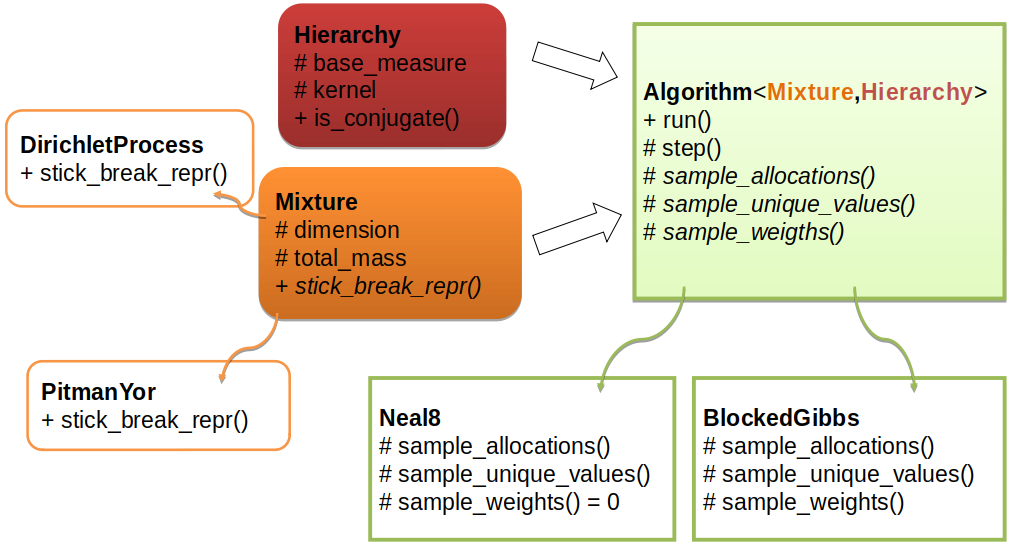
\includegraphics[width=\linewidth]{etc/code_map.png}
\end{frame}
